\section{Background}

In this section, we first introduce the process of agentic RL training in \S\ref{sec:background_rl}.
Then we discuss the external resource management in \S\ref{sec:background_resource}, followed by the over-provisioning analysis in \S\ref{sec:background_op}.
Finally, we present our opportunities and challenges of external resource management in \S\ref{sec:background_opp}

\subsection{Agentic RL Training}
\label{sec:background_rl}
Agent shows significant performance improvement in handling real-world problems, including AI coding, deep searching, and embodied AI~\citep{dou2024stepcoder,qi2025webrl,wang2023voyager}.
Unlike traditional LLM, agentic LLM can interact with the real world through external tools, e.g., shell commands, APIs, or device operations.
The usage of external tools makes the RL pipeline of the agentic LLM different from the traditional LLM.
% Therefore, we need agentic RL as an important part during post-training.


\begin{figure}[t]
    \centerline{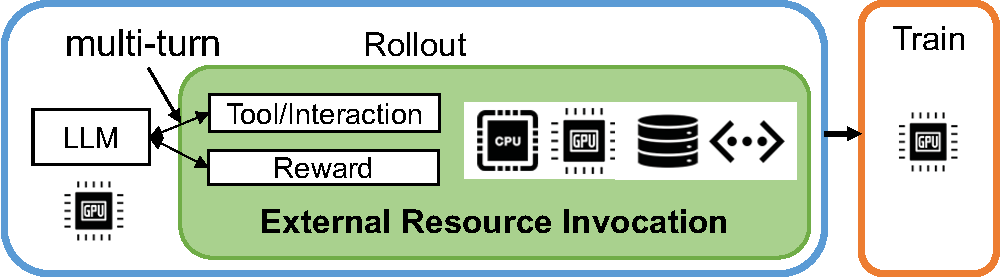
\includegraphics[width=0.7\linewidth]{figures/background_workflow.pdf}}
    \vspace{-0.1in}
    \caption{One training step of agentic RL.}
    \label{fig:background_workflow}
    \vspace{-0.2in}
\end{figure}

Agentic RL pipeline is illustrated in Figure~\ref{fig:background_workflow}. Given a batch of samples, the RL framework first uses an agentic LLM to process the samples and collects their execution trajectories, a phase known as \textit{rollout} in RL.
During the rollout phase, the framework typically follows the ReAct pattern~\citep{yao2022react}, 
where the LLM decides how to use tools based on the input prompt, then the RL framework accordingly performs tool invocations and gets the observation of the environment. 
Once a trajectory is completed, its reward is calculated based on either preference (e.g., RLHF~\citep{ouyang2022training} and LLM-as-a-judger~\citep{bai2022constitutional}) or ground-truth (e.g., RLVR~\citep{guo2025deepseek}), and subsequently used to train LLM.
% a loop of LLM generation and tool calling/environment interaction.
% First, the RL framework uses the LLM to decide how to use the tools based on the input prompt.
% Then, the RL framework performs tool invocations according to the LLM response and gets the observation of the environment.
% The observation is forwarded to the LLM for further decision.

Within a single trajectory, instead of invoking tools only once,  agentic RL usually repeats the ReAct pattern over multiple turns to enhance LLM's capacity of tool usage. 
While generation and training of LLM primarily consume GPU resources, tool invocations rely on heterogeneous resource types including CPU, GPU, storage, and network, termed as \textbf{external resources}  from the perspective of the RL framework.
Further, frequent invocations for external resources are a pronounced characteristic of agentic RL.
For example, AI coding repeatedly executes shell commands or edits files using CPUs, while DeepSearch accesses multiple websites and consumes API quotas.
In addition, reward computation at the end of trajectories typically involves external resources as well: LLM-as-a-judge is commonly deployed as an independent model service, and AI coding evaluates rewards by running a large amount of test cases.
All such operations that invoke resources outside the RL framework can be collectively referred to as \textbf{external resource invocations}. 

% Besides, reward services requiring GPUs to calculate the reward scores are becoming a trend~\citep{mopd,}


% The RL job generally falls into two categories: synchronous and asynchronous.
% For the synchronous RL, the training process occurs only after collecting the trajectories of every sample.
% The serial execution of synchronous RL introduces severe straggler bottlenecks: a single slow sample stalls the entire RL job.
% Conversely, asynchronous RL decouples the rollout phase and the training phase, allowing independent rollout phase while the training phase continuously consumes buffered collected samples.
% Asynchronous RL avoids the straggler problem, especially for agentic RL tasks, making it widely used in practice~\citep{}.

\subsection{External Resource Management}
\label{sec:background_resource}

% Although the demands for external resource invocations are urgent and general, there remain requirements for extra management efforts, because of three reasons.
Agentic RL training requires external resources to hold the environments, tools, or reward services.
The external resources require additional management efforts mainly due to two reasons, i.e., RL efficiency and resource cost.

% \xin{Add references or some experiment figures to support the three issues. You cannot just claim the issues without any evidence.}
% \xbj{TODO: add two figures, merge 1 and 3}


First, the efficiency of RL tasks is highly related to how well the external resources are used.
Intuitively, if the external resource is insufficient or allocated inappropriately, the execution duration of external invocation is lengthened.
Note that, according to the commonly used agentic RL workflow in \S\ref{sec:background_rl}, the external invocations are all on the critical path of the rollout for each sample.
Thus, longer external invocations indicate longer rollout, and also longer RL training.
For example, we evaluate the same RL task under different amount of external resources.
Figure~\ref{fig:motiv_sm}(a) illustrates that the RL task with inappropriate external resources (0.5$\times$) has longer average ACT and step duration than the RL task with 1$\times$ resources.
More severely, if too many external invocations fail, the RL training task may also fail~\citep{jiang2025verltool}.

Second, the external invocations introduce additional resource cost, and it is highly motivated to reduce costs of external resources.
Usually, agentic RL requires deploying a CPU cluster for environment construction, or specialized GPUs that provide reward service for RL training, leading to extra expenses.
For example, a newly proposed distillation workflow, MOPD~\citep{xiao2026mimo}, uses dozens of teacher models with hundreds of GPUs to get the reward for one RL task.
% Approximately, MOPD leads to about xx\% additional GPU cost.
However, these external GPUs are not fully utilized.
Figure~\ref{fig:motiv_sm}(b) shows the SM activity of GPUs used by 12 teacher models.
The SM activity vibrates among time dimension and model dimension with an average less than 3\%,
which demonstrates great waste of external resources.


\begin{figure}[t]
    \begin{minipage}{0.24\linewidth}
        \centerline{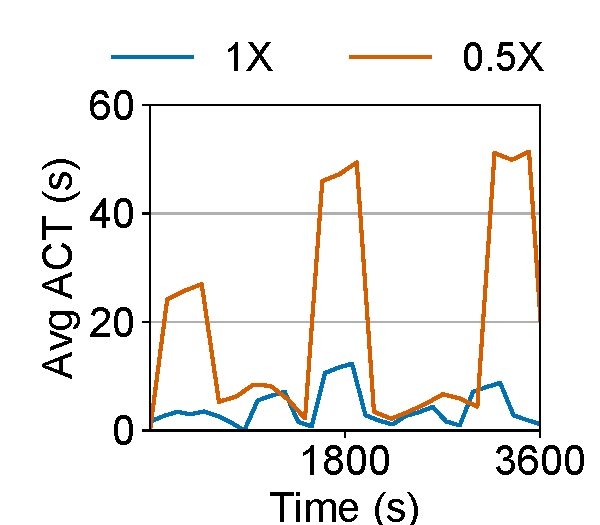
\includegraphics[width=\linewidth]{figures/Motiv_code_act.pdf}}
        % \vspace{-0.15in}
        \centerline{\small \quad(a)}
        % \vspace{-0.1in}
    \end{minipage}
    \begin{minipage}{0.24\linewidth}
        \centerline{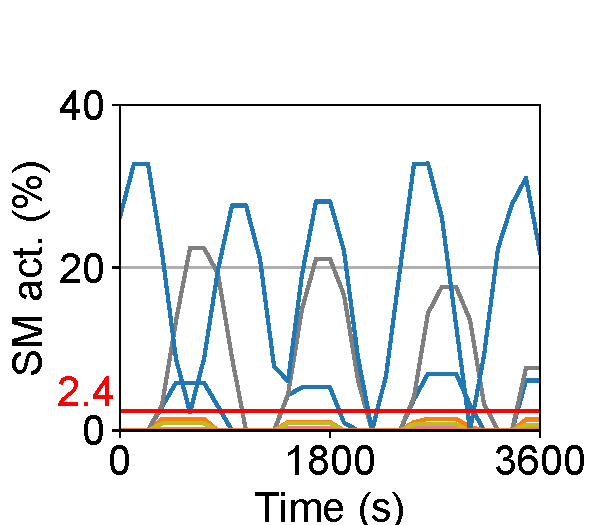
\includegraphics[width=\linewidth]{figures/Motiv_mopd_sm.pdf}}
        % \vspace{-0.15in}
        \centerline{\small \quad(b)}
        % \vspace{-0.1in}
    \end{minipage}
    \begin{minipage}{0.24\linewidth}
        \centerline{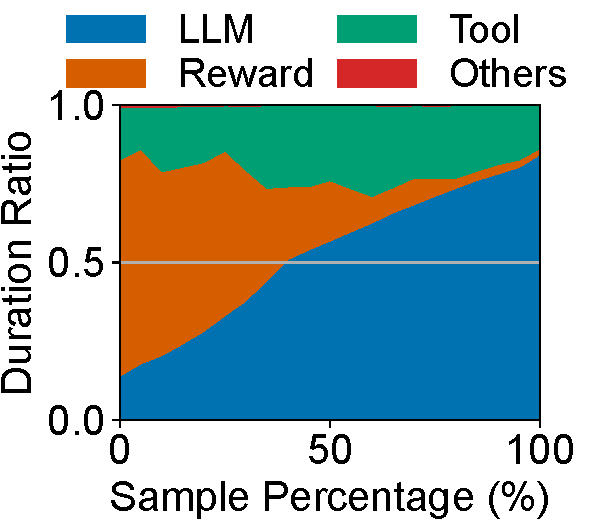
\includegraphics[width=\linewidth]{figures/Motiv_traj_code.pdf}}
        % \vspace{-0.15in}
        \centerline{\small \quad(c)}
        % \vspace{-0.1in}
    \end{minipage}
    \begin{minipage}{0.24\linewidth}
        \centerline{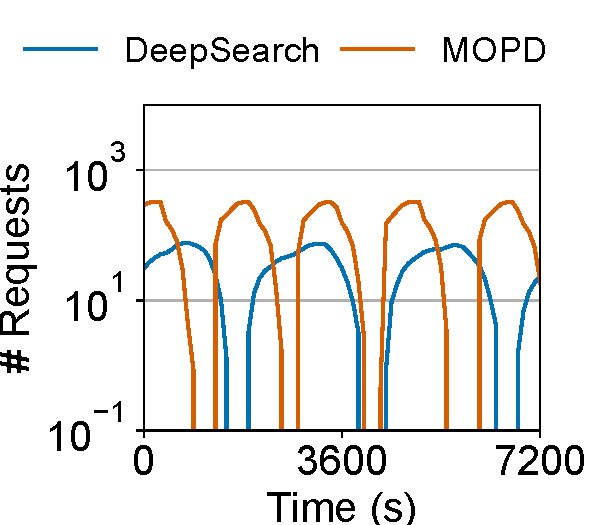
\includegraphics[width=\linewidth]{figures/Motiv_req_counts.pdf}}
        % \vspace{-0.15in}
        \centerline{\small \quad(d)}
        % \vspace{-0.1in}
    \end{minipage}
    \vspace{-0.1in}
    \caption{(a): average ACT under 1$\times$ and $0.5\times$ external resource quantities. (b): SM activity of 12 different reward services in MOPD. (c): Code agent rollout duration ratio. (d): \# External invocations of two agentic RL tasks.}
    \label{fig:motiv_sm}
    \vspace{-0.2in}
    \end{figure}
\iffalse
First, 
%agentic RL introduces substantial \textit{resource cost}.
the external resource invocations introduce additional training cost, and it is highly motivated to reduce costs of external resources.
% According to our in-house experience, the cost stemmed from external resources can be up to xx\% of the training cost.
For example, deploying a Kubernetes cluster with computers of specialized versions, or several nodes of high-performance GPUs that completely provide service for RL training, leads to substantial expenses. 
Especially, a new proposed pipeline of integrating different models tuned with RL, MOPD~\citep{xiao2026mimo}, uses a student model to rollout trajectories of different tasks (including agentic RL tasks) and correspondingly align with teachers. This pipeline requires deploying dozens of teacher models as reward services, each of which is equipped with several nodes in the GPU cluster. The total expenses are quite costly.



Second, the \textit{GPU efficiency} of RL tasks is related to the external resource usage.
According to the agentic RL training workflow described in \S~\ref{sec:background_rl}, each interaction between RL task and external resources lies on the critical path of the \textit{rollout} phase, plummeting the GPU efficiency of RL task.
% Meanwhile, compared with traditional RL training, the generation batch size on each data-parallel (DP) group is typically small (often no more than 64, and sometimes significantly less) due to the substantially longer trajectories in agentic settings.
Meanwhile, considering the substantially longer trajectories in agentic RL than traditional RL, the generation batch size on each data parallel (DP) group of agentic RL  is typically small, e.g., no more than 64.
As a result, the inference engine often fails to fully saturate GPUs during the decoding stage.
Once a subset of trajectories enters the tool-calling phase, the number of active trajectories in LLM decoding decreases, which directly reduces the inference batch size. 
According to the roofline model~\citep{}, this leads to a noticeable drop in GPU utilization.
%particularly in terms of streaming multiprocessor (SM) occupancy and memory bandwidth efficiency. 
Therefore, inefficient management of external resources not only wastes external resources but also indirectly degrades the GPU utilization of RL tasks.

Third, the \textit{training stability} can be influenced by the external resource usage.
When external tools crash or time out, e.g., due to API rate limits or queued tool invocations, the RL training jobs collapse. Even if these errors occur occasionally, they will cause the trajectory to be ineffective, reducing the passrate of RL training and prolonging the rollout phase.
\fi

Existing frameworks~\citep{sheng2025hybridflow,fu2025areal,wang2025let} either overlook these interdependencies or default to static over-provisioning, leading to severe resource waste and cost inefficiency.

\subsection{Over-Provisioning of External Resources}
\label{sec:background_op}
% Existing works, along with some trivial approaches, 
The over-provisioning of external resources during agentic RL training can be categorized into two levels, both of which exacerbate training inefficiency and resource waste.

\parabf{Over-provisioning within trajectories.}
% Within a single trajectory, agents typically reserve or assume the availability of external resources (e.g., simulators, databases, search engines, or specialized inference services) for the entire duration of the rollout. However, actual interactions with these resources only occur at a small subset of time steps. As a result, resources remain idle for most of the trajectory execution, leading to low utilization and unnecessary blocking of other concurrent requests.
To guarantee the continuity and independence of multi-turn invocations, some agentic RL tasks require an isolated environment for each trajectory to interact with during the \textit{rollout} phase.
Existing frameworks~\citep{kubernetes}, statically allocate external resources for the entire lifecycle of a trajectory, although the trajectory only interacts with these resources within some time windows. 
We use a typical RL task in production, AI coding, to evaluate the action duration (including tool calling and reward calculation) of each trajectory.
As shown in Figure~\ref{fig:motiv_sm}(c), the time ratio of each trajectory is only 47\% on average. 

% Unlike the diagram, the distribution of LLM generation and environment invocation is not continuous. Instead, they are interleaved in the trajectory.
In practice, the LLM generation and external invocation phases are interleaved.
However, existing systems create environments and reserve external resources during the whole rollout phase.
% at the beginning of the trajectory and release them only after the trajectory terminates.
As a result, the reserved resources remain idle for most of the time, wasting resources that could otherwise be used by other trajectories. 
For example, the wasted external resources count for 53\% for AI coding (Figure~\ref{fig:motiv_sm}(c)).
% Consequently, a much larger CPU cluster is required to guarantee the stability and scale of agentic RL training, posing more severe challenges to both cluster scalability and cost efficiency.

Moreover, under finite external resources, over-provisioning within trajectories significantly limits system concurrency, increases queueing delays for tool invocations, and prevents allocating additional resource units to extremely computation-intensive operations.
These effects prolong rollout time and further reduce the overall efficiency of RL frameworks, as well as the utilization of GPUs in the training cluster.

% \begin{figure}[t]
%     \begin{minipage}{0.48\linewidth}
%         \centerline{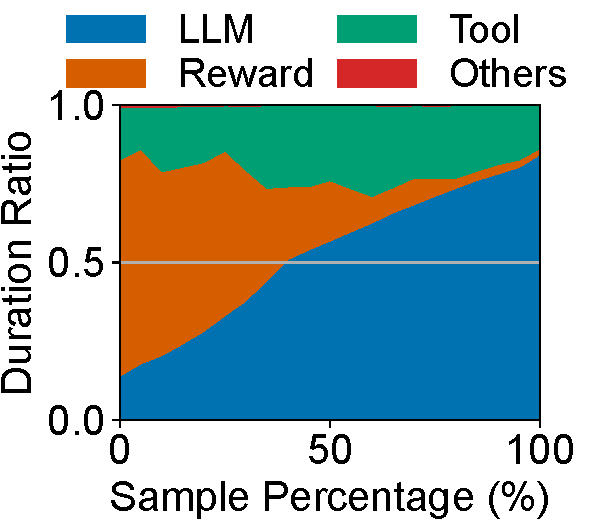
\includegraphics[width=\linewidth]{figures/Motiv_traj_code.pdf}}
%         % \vspace{-0.15in}
%         % \centerline{\small (a).}
%         % \vspace{-0.1in}
%     \end{minipage}
%     \begin{minipage}{0.48\linewidth}
%         \centerline{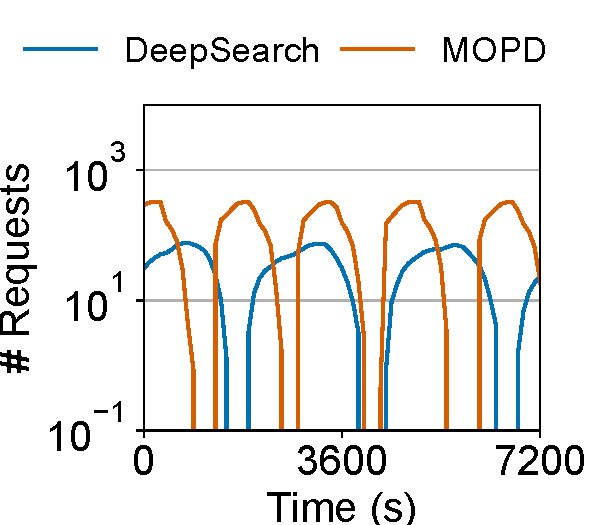
\includegraphics[width=\linewidth]{figures/Motiv_req_counts.pdf}}
%         % \vspace{-0.15in}
%         % \centerline{\small (b).}
%         % \vspace{-0.1in}
%     \end{minipage}
%     \vspace{-0.1in}
%     \caption{Left: Code agent rollout duration ratio. Right: \# External invocations of two agentic RL tasks.}
%     \label{fig:motiv_op}
%     \vspace{-0.2in}
%     \end{figure}

\parabf{Over-provisioning within RL tasks.}
At the task level, different RL tasks usually require different external services to interact or calculate reward because of the service type and configuration~\citep{li2025cuda,jin2025search,xiao2026mimo}.
For example, different RL tasks that use reward models often send requests to separate reward services, because these models may differ in model architecture or parameters. 
These external services are usually deployed with different external resources~\citep{micromulti,jiang2025verltool}.

However, the external services are not fully used all the time, mainly because of the dynamism of external invocations along the entire RL training process.
For each RL task, there are even no external invocations during the training phase, leaving idle external services.
% Even during the rollout phase, the external invocations fluctuate considering the dynamism.
We profile the number of external invocations of two real agentic RL tasks, DeepSearch and MOPD, as shown in Figure~\ref{fig:motiv_sm}(d).
Note that the number of invocations varies up to three orders of magnitude, leading to severe waste of external resources.

% Apart from isolated environments for trajectories, agentic RL tasks also invoke various external services for consulting or judging.
% % The existence of over-provisioning within RL tasks is orthogonal to that within trajectories. In practice, 
% Therefore, they are usually provisioned with isolated clusters for external resource invocations, even when they rely on the same type of external resources.
% For example, different RL tasks that use reward models often send requests to separate reward services, because these models may differ in model architecture or parameters. 

% However, the utilization of external resources fluctuates significantly within a single RL task, in addition to within individual trajectories. Figure~\ref{fig:motiv_op}(b) illustrates the number of reward requests during the RL training of the DeepSearch Agent, and the number varies dramatically with the training proceeding. Due to the phase alternation between generation and training in many existing RL frameworks~\citep{sheng2025hybridflow,gao2025rollpacker}, interactions with external resources are blocked during the training phase. Consequently, the provisioned resources for this task remain idle for extended periods, resulting in severe resource waste.

\subsection{Opportunities and Challenges}
\label{sec:background_opp}
% According to the Agentic RL training pipeline described in section~\ref{}, each action to interact with external resources is on the critical path of \textit{rollout}. Meanwhile, during agentic RL training, the generation batch size on each data parallel (DP) group are relatively small compared with common RL training (usually 64 or even less, thus the inference engine fails to saturate the GPUs in the decoding stage), due to much longer lengths of trajectories. Therefore, once a trajectory begins to interact with external resources, the number of trajectories that are running in the inference engine decreases. Due to the existence of roof line model, the utilization of GPUs, i.e., SM utilization, decreases as well. 

\parabf{Opportunities in Action-level Scheduling.}
To address the inefficiency caused by the aforementioned over-provisioning, we propose to manage external resources at the \textbf{action-level}. 
Here, an \textit{action} refers to an atomic invocation of external resources, during which neither LLM generation nor any other actions in the trajectory are interleaved.

%implicitly 
Instead of allowing each trajectory to independently perform external invocations and reserve resources, all actions are submitted to a unified system that centrally manages heterogeneous external resources. 
In this system, invocations with the long-lived environments or services are uniformly scheduled and managed in the granularity of actions, i.e., \textbf{Breakdown} the resource occupation of long-lived environments/services. 
Further, the system uses pooled resources to serve these actions, and elastically allocates resources among them, i.e., \textbf{Pool} the resources. 
Through the process of \textbf{Breakdown} \& \textbf{Pool}, the over-provisioning problem is eliminated by the action-level scheduling, because the external resources are released or shrunk during the idle time.
% caused by LLM generation within trajectory or \textit{train} phases within RL tasks.
% Upon receiving an action request, the platform schedules its execution and elastically allocates reasonable resources based on the current system state (including resource availability, queue lengths, and contention levels) as well as the properties of the action (including predicted execution duration, resource type, and scalability). The execution result is then returned to the agentic RL framework and dispatched to the corresponding trajectory, enabling the alternating loop between LLM generation and tool invocation to proceed.

In addition to mitigating over-provisioning, action-level scheduling enables more flexible and fine-grained resource allocation, compared with the trajectory-level or task-level resource allocation in the past.
% The scheduler can assign the minimum required amount of resources tailored to each action, avoiding waste when the resource requirement of a certain action is extremely higher than others in a trajectory.
% Moreover, 
For example, when sufficient resources are available, it can dynamically allocate additional resource units to elastic actions, i.e., increase the degree-of-parallelism (DoP), to shorten execution durations, thereby further improving overall RL training efficiency.

In conclusion, by refining the granularity of resource management from trajectories or RL tasks to individual actions, action-level scheduling could:
(i) reduce resource idle time caused by long inactive periods through multiplexing across trajectories and tasks; and
% (ii) allocate resource units that are specifically matched to the requirements of each action; and
(ii) shorten interaction latency by dynamically scaling resource allocation.




\parabf{Challenges.}
% \xbj{exemplify heterogeneity? Additionally, although there is a unified abstraction modeling, heterogeneous resources and job patterns still challenge the generalizability. 
First, although action-level scheduling simplifies the workflow of individual actions, the diversity of resources and interaction patterns still poses difficulties in unified management (\S\ref{sec:design_modeling}). 
% For example, for some resources and job patterns, the execution duration is easy to predict, like the inference of reward models on GPUs. We can roughly predict the duration of a request through its input length along with the placement of targeted reward model. Instead, the extremely sophisticated scenarios on CPUs lead to the unpredictability of the execution durations for all CPU programs, among which only a small part of specific jobs with similar properties can be predicted in advance.
There are multiple external resources managed in the system, and an action may utilize more than one resource types. It is challenging to uniformly orchestrate these resources.
In addition, the patterns of actions, in terms of elasticity and execution durations, vary as well.
Therefore, designing a general abstraction, together with a set of unified interfaces to manage heterogeneous resources, is an essential foundation for building a unified scheduling algorithm.

Second, the scheduler must handle diverse and bursty workloads (\S\ref{sec:design_scheduling}).
Designing a unified and efficient scheduling algorithm under these conditions is challenging, since existing algorithms~\citep{grandl2016graphene,han2022microsecond,liu2024muxflow} are usually tailored to specific domains and do not generalize well to heterogeneous resources and job patterns.
Furthermore, the relatively short execution durations of actions (e.g., down to 1ms in AI coding) leave a quite short window for scheduling, making it impractical to apply heavyweight optimization techniques. %such as machine learning–based or convex optimization–based schedulers.

Third, enabling action-level scheduling requires decoupling resource allocation from long-lived stateful environments or services (\S\ref{sec:design_resource_managing}). Over-provisioning within trajectories/tasks originates from the need to maintain persistent state throughout an entire trajectory/task.
Therefore, a key challenge lies in how to release resources after each action while preserving the state of the environment/service and supporting real-time resource allocation and fast state restoration. 
% 2. efficient temporal multiplexing of external resources, reduce the overhead of multiplexing
In addition, it is non-trivial to support elastic DoP and dynamic resource scaling for heterogeneous resources with diverse characteristics and topologies.

% Finally, many existing approaches focus primarily on job reordering~\citep{} rather than elastic resource allocation, while both overly aggressive and overly conservative scaling strategies can lead to suboptimal interaction latency and degraded training efficiency.
